\documentclass[a4paper, 12pt]{article}
\usepackage{graphicx}
\usepackage{enumitem}
\usepackage{mathtools}
\usepackage{hyperref}
\usepackage{caption}
\usepackage{subcaption}
\def\code#1{\texttt{#1}}
\def\f#1{Figure \ref{fig:#1}}
\begin{document}

\title{\vspace{4.0cm}Applied GPU Programming - Assignment II\\
\large DD2360 HT20}
\author{Pontus Asp}
\date{\today}
\maketitle
\thispagestyle{empty}
\pagenumbering{roman}
\newpage

\clearpage
\pagenumbering{arabic}

% Write here ->
\section{Git repository}
I uploaded my git repository to GitHub. I use the same git repository for the entire course but the folder structure requested is still followed under the root folder. I also have 2 extra directories, one for this report and one where I have code from lectures.
\\\\
Here is the link to my git repository:\\
\url{https://github.com/pontusasp/kth-dd2360/tree/master/Assignment_2}


% 1. Explain how the program is compiled and the environment that you used.

% 2. Explain what are CUDA threads and thread blocks, and how they are related to GPU execution.
\section{Exercise 1}
My output from my program was \code{Hello World! My threadId is \%d}, where \code{\%d} was the thread id. The prints did not come in the "right" order, but that was according to my expectations, since the execution on the GPU is in parallel. I compiled my source code with the \code{nvcc} command without any special parameters (\code{nvcc exercise\_1.cu -o bin/out}). I compiled and ran my software in Ubuntu 20.04 and used a Nvidia GeForce GTX 1070 graphics card.\par CUDA Threads are threads running the functions on the GPU (kernels). When you launch a kernel from the code, you specify how many thread blocks and how many threads per block that the GPU should do the work with. The number of CUDA Threads is the number of thread blocks times the number of threads per block, and each and everyone of these threads will run the kernel.


% Explain how you solved the issue when the ARRAY_SIZE is not a multiple of the block size. If you implemented timing in the code, vary ARRAY_SIZE from small to large, and explain how the execution time changes between GPU and CPU.
\section{Exercise 2}
I solved the issue of the \code{ARRAY\_SIZE} not being a multiple of the \code{BLOCK\_SIZE} by using the method mentioned in the lecture material, namely by doing \code{(ARRAY\_SIZE + BLOCK\_SIZE - 1) / BLOCK\_SIZE}. This works with the help of integer division, which makes \code{(BLOCK\_SIZE - 1) / BLOCK\_SIZE} equal zero. So then we can make sure that if \code{ARRAY\_SIZE} is not a multiple of the block size we get one extra CUDA thread per block to make up for it so we will not miss any of the work.
\par When varying the \code{ARRAY\_SIZE} from small to large I could see that the smaller it was the better the CPU performed against the GPU. While increasing the size of the \code{ARRAY\_SIZE} the GPU performed better compared to the CPU the bigger it was. This is because of the latency of launching kernels and transferring data to the GPU. This means that if the amount of parallelization possible is small (for instance a small amount of data that should be processed) the GPU usually performes worse than the CPU, while the opposite is true if the amount of parallelization possible is a lot. The small vs large \code{ARRAY\_SIZE} is a good example of this.




\section{Exercise 3}
% 1. Measure the execution time of the CPU version, varying the number of particles.

% 2. Measure the execution time of the GPU version, varying the number of particles, like in 1).
% 2.1. Include data copying time to and from in the measurement.
% 2.2. For each GPU particle configuration, vary the block size in the GPU version from 16, 32, …, up to 256 threads per block.

% 3. Generate one or more performance figures based on your measurements in 1 and 2. Include it in the report with a description of the experimental setup (e.g., GPU used) and the observations obtained from the results. Explain how the execution time of the two version changes when the number of particles increases. Which block size configuration is optimal?

% 4. Currently, the particle mover is completely offloaded to the GPU, only with data transfer at the beginning and end of the simulation. If the simulation involves CPU dependent functions (i.e. particles need to be copied back and forth every time step), would your observation in 3) still holds? How would you expect the performance will change in terms of GPU execution? Make an educated guess using the GPU activities timing provided by nvprof.
I did a number of different test runs on the CPU and GPU. Each time measured in the graphs is an average out of five test runs measured with the system clock directly in the programs. I ran these tests on my home PC which runs on a Nvidia GeForce GTX 1070 graphics card and an Intel Core i7 7700k processor, the OS used was Ubuntu 20.04.
\par The observations I made when the number of particles was increasing was that both the CPU and GPU of course had an increased execution time. However the execution time was increasing drastically faster on the CPU than the GPU. If we compare the 10k particle run on the CPU (\f{ex-3-cpu}) and the 10k particle run on the GPU (\f{ex-3-gpu-10k}) the execution times does not differ that much. However if we look at the 10000k (10 M) run we can see that there is a big difference between the execution time of the CPU (\f{ex-3-cpu}) and the GPU (\f{ex-3-gpu-10000k}).
\par In the GPU graphs there are also 5 different measurements for a few different block sizes. In these tests it is clear that there is no clear optimal block size. For insteance in the 10k run in \f{ex-3-gpu-10k} the optimal block size is 128, and the worst one is 16, while if we look at \f{ex-3-gpu-10000k} the results are the opposite. Out of the 4 different graphs the only ones that seem to agree on the performance of the different block sizes are \f{ex-3-gpu-100k} and \f{ex-3-gpu-1000k}.
\par If the simulation could not be fully offloaded to the GPU but some parts had to be calculated on the CPU then I am guessing that the observations made here would not hold. If we for instance needed to copy data from the GPU to the CPU between every simulation step then the memory copy and latency would become much more apparent and slow the program down a lot compared to only copying the data in the start and the end. We would probably need to synchronize the code as well which could also slow down the progression.
\begin{figure}
    \centering
	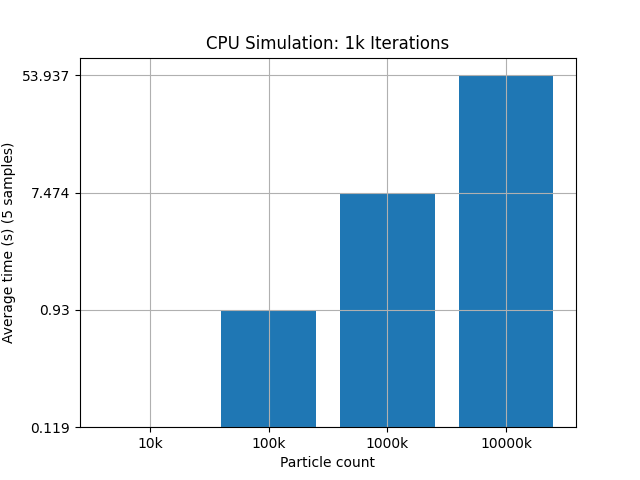
\includegraphics[width=0.8\linewidth]{graphs/ex_3_graph_cpu.png}
	\caption{CPU measurements.}
    \label{fig:ex-3-cpu}
\end{figure}

\begin{figure}
    \centering
    \begin{subfigure}{.5\textwidth}
      \centering
      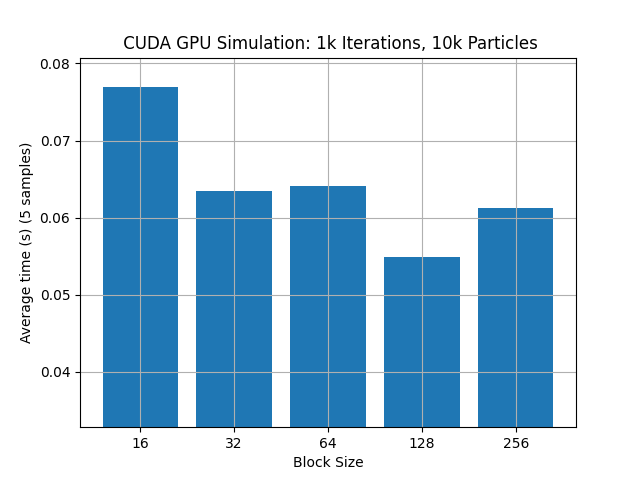
\includegraphics[width=1\linewidth]{graphs/ex_3_graph_gpu_10k.png}
      \caption{10k}
      \label{fig:ex-3-gpu-10k}
    \end{subfigure}%
    \begin{subfigure}{.5\textwidth}
      \centering
      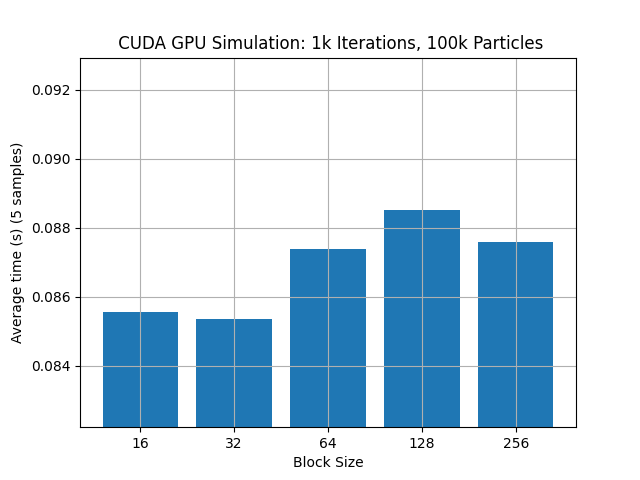
\includegraphics[width=1\linewidth]{graphs/ex_3_graph_gpu_100k.png}
      \caption{100k}
      \label{fig:ex-3-gpu-100k}
    \end{subfigure}
    \caption{GPU measurements for 10k and 100k particles.}
    \label{fig:test}
\end{figure}

\begin{figure}
    \centering
    \begin{subfigure}{.5\textwidth}
      \centering
      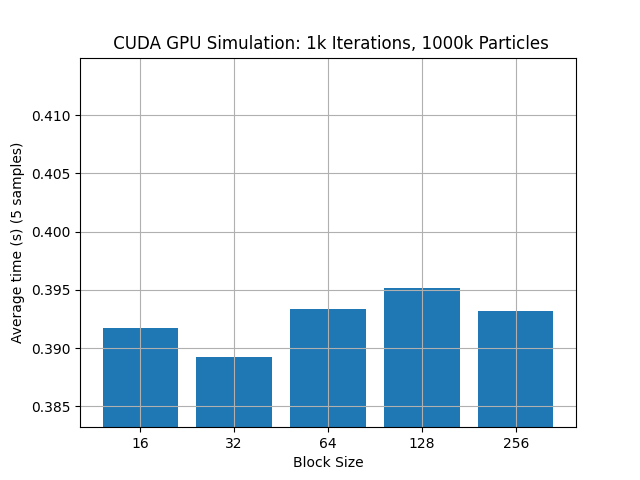
\includegraphics[width=1\linewidth]{graphs/ex_3_graph_gpu_1000k.png}
      \caption{1000k}
      \label{fig:ex-3-gpu-1000k}
    \end{subfigure}%
    \begin{subfigure}{.5\textwidth}
      \centering
      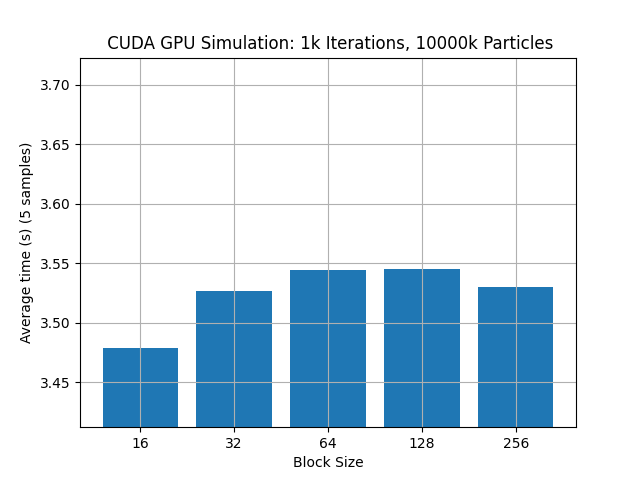
\includegraphics[width=1\linewidth]{graphs/ex_3_graph_gpu_10000k.png}
      \caption{10000k}
      \label{fig:ex-3-gpu-10000k}
    \end{subfigure}
    \caption{GPU measurements for 1000k and 10000k particles.}
    \label{fig:test}
\end{figure}

% 1. Measure the execution time of the GPU version, varying NUM_ITER.

% 2. Measure the execution time, varying the block size in the GPU version from 16, 32, …, up to 256 threads per block.

% 3. Change the code to single precision and compare the result and performance with the code using double precision. Do you obtain what you expected in terms of accuracy and performance? Motivate your answer.
\section{Bonus Exercise}




% Write here <--

\end{document}